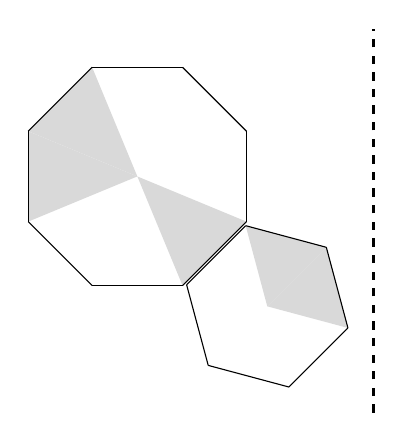
\begin{tikzpicture}[scale=0.75]
\def\radius{2}
\def\smallradius{1.414}
\foreach \angle [count=\i] in {0,45,...,315} {
\coordinate (A\i) at (\angle+22.5:\radius);
}
\foreach \i [remember=\i as \lasti (initially 8)] in {7} {
\fill[gray!30] (0,0) -- (A\i) -- (A\lasti) -- cycle;
}
\foreach \i [remember=\i as \lasti (initially 5)] in {4,3} {
\fill[gray!30] (0,0) -- (A\i) -- (A\lasti) -- cycle;
}

\foreach \i [remember=\i as \lasti (initially 8)] in {1,...,8} {
\draw (A\lasti) -- (A\i);
}
\begin{scope}[shift={(2.2,-2.2)}]
\foreach \angle [count=\i] in {0,60,...,300} {
\coordinate (B\i) at (\angle+45:\smallradius);
}
\foreach \i [remember=\i as \lasti (initially 6)] in {1,2} {
\fill[gray!30] (0,0) -- (B\i) -- (B\lasti) -- cycle;
}
\foreach \i [remember=\i as \lasti (initially 6)] in {1,...,6} {
\draw (B\lasti) -- (B\i);
}
\end{scope}
\draw[dashed,thick] (4,-4) -- (4,2.5);
\end{tikzpicture}